\documentclass[a4paper]{article}
\usepackage{fuzz}
\usepackage{graphicx}

\begin{document}
\section{Introduction}
This is another version of the watergate example with usage of an
$Invariant$ schema. Here we moved some safety properties 
from the state schema to the $Invariant$ schema,
so each operation must ensure that the safety properties are
fullfilled. 

Model checking can be used to check if there is a flaw in the specification.

\section{Static configuration of the system}
Here we describe the components of the system which won't change
during the operation of the watergates.

Normally we would specify the pools and gates as given sets. But
to simplify the animation of a certain model, we explicit name each pool
and gate.
\begin{zed}
  POOL ::= pool1 | pool2 | pool3 | pool4 | pool5\\
  GATE ::= gate1 | gate2 | gate3 | gate4
\end{zed}

\begin{center}
  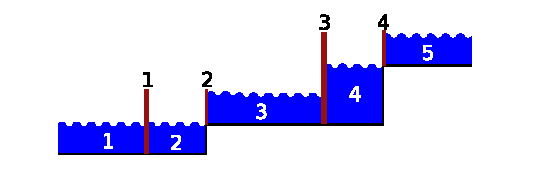
\includegraphics{watergateillustration}
\end{center}

\subsection{The pools}
Every pool has a minimum and maximum gauge. Rivers and canals
whose gauge is not under control of the system, have the same
maximum and minimum gauge. \emph{mingauge} and \emph{maxgauge}
wouldn't are given explicit to simplify animation.

\begin{axdef}
  mingauge, maxgauge : POOL \fun \nat\\
  \where
  \forall p : POOL @ mingauge~p \leq maxgauge~p\\
  mingauge = \{(pool1,1), (pool2,1), (pool3,2), (pool4,2), (pool5, 4)\}\\
  maxgauge = \{(pool1,1), (pool2,2), (pool3,2), (pool4,4), (pool5, 4)\}\\
\end{axdef}

\subsection{The gates}
Every gate connects two pools. As above the explicit connections are
given to simplify the animation.

\begin{axdef}
  connect : GATE \fun (\power POOL)
  \where
  \forall r : \ran connect @ \# r = 2\\
  connect = \{
  (gate1, \{pool1, pool2\}),
  (gate2, \{pool2, pool3\}),\\\\
  \t1 (gate3, \{pool3, pool4\}),
  (gate4, \{pool4, pool5\})\}
\end{axdef}

\section{State of pools and gates}
Each pool has a current gauge.
We save the set of opened gates, all other gates are closed. 

\begin{schema}{State}
  gauge : POOL \fun \nat\\
  opengates : \power GATE\\
\end{schema}

\subsection{Invariant}

The gauge of each pool is between its minimum and maximum.
If a gate is open, the pools on both sides of the gate must have the same gauge.
This property must not be violated by any operation.

\begin{schema}{Invariant}
  State
  \where
  \forall p : POOL @ mingauge(p) \leq gauge(p) \leq maxgauge(p)\\
  \forall g : opengates; p1,p2 : POOL | connect~g = \{p1, p2\} \\\\
  \t1 @ gauge(p1) = gauge(p2)\\
\end{schema}


\section{Operations on the state}

\subsection{Opening and closing of the gates}
An Operation on the gates doesn't change the gauges of the pools. Every
Operation takes an gate as an argument.
\begin{schema}{GateOperation}
  \Delta State\\
  gate? : GATE\\
  \where
  gauge' = gauge
\end{schema}
It's possible to close an open gate everytime.
\begin{schema}{Close}
  GateOperation
  \where
  gate? \in opengates\\
  opengates' = opengates \setminus \{ gate? \}
\end{schema}
It's only possible to open closed gates when the gauge of the pools
on both sides of the gate is the same.
\begin{schema}{Open}
  GateOperation\\
  \where
  gate? \notin opengates\\
  opengates' = opengates \cup \{ gate? \}\\
  \forall p1,p2 : POOL | connect~gate? = \{p1,p2\} @ gauge~p1 = gauge~p2
\end{schema}

\subsection{Raising and lowering of the gauges}
An Operation on the pools does not change the state of the gates.
It's only possible to lower or raise pools, which gates are all
closed.
\begin{schema}{PoolOperation}
  \Delta State\\
  pool? : POOL
  \where
  opengates' = opengates\\
  \forall g : opengates @ pool? \notin connect~g\\
\end{schema}
It's only possible to raise the gauge of a pool if it's maximum is
not reached yet.
\begin{schema}{Raise}
  PoolOperation\\
  \where
  gauge(pool?) < maxgauge(pool?)\\
  gauge' = gauge \oplus \{pool? \mapsto gauge(pool?) + 1\}\\
\end{schema}
It's only possible to lower the gauge of a pool if it's minimum is
not reached yet.
\begin{schema}{Lower}
  PoolOperation\\
  \where
  gauge(pool?) > mingauge(pool?)\\
  gauge' = gauge \oplus \{pool? \mapsto gauge(pool?) - 1\}\\
\end{schema}
  

\section{Initialisation}
The systems starts in a state where all gates are closed and
all the water gauges are on the minimum.
\begin{schema}{Init}
  State'
  \where
  gauge' = mingauge\\
  opengates' = \emptyset\\
\end{schema}

\end{document}
